\subsection{Field-identified tissue comparisons}\label{sec:field}

All seven retained objects completed seven procedures at each of three seeds (147 method--seed runs). Independent raw-HDF5 checks reproduce selected cells, fields and reference labels; rescoring saved predictions reproduces every ARI. All stored spatial graph edges are within field. Table~\ref{tab:field-inputs} gives the physical and annotation counts; Table~\ref{tab:field-ari} gives the raw named-method readouts. This is a completed reanalysis of the explicitly retained scope, not the earlier pilot and not a replacement for every historical method or dataset.

\begin{table*}[!htbp]\centering\small

\caption{New field-identified panel. Cell and field counts refer to the actual model inputs; label counts exclude missing/unknown reference labels. $C$ averages within-field labelled-neighbour agreement over cells with neighbours. $C_0$ is the field-preserving permutation expectation; adjusted $C$ equals $(C-C_0)/(1-C_0)$. CODEX niche annotations are cluster-derived proxies, not independent biological labels.}

\label{tab:field-inputs}

\begin{tabular}{lrrrrrrr}\toprule

Object & Cells & Labelled & Fields & Classes & $C$ & $C_0$ & adjusted $C$\\\midrule

DLPFC & 3,639 & 3,611 & 1 & 7 & 0.905 & 0.181 & 0.884\\

MERFISH & 5,488 & 5,488 & 1 & 8 & 0.931 & 0.174 & 0.917\\

STARmap & 1,207 & 1,207 & 1 & 7 & 0.921 & 0.162 & 0.906\\

MIBI & 3,309 & 3,309 & 3 & 8 & 0.486 & 0.213 & 0.348\\

Open-ST & 15,000 & 13,420 & 1 & 14 & 0.562 & 0.183 & 0.464\\

CODEX & 16,000 & 15,454 & 565 & 100 & 0.120 & 0.086 & 0.038\\

Zhuang & 16,000 & 16,000 & 1 & 17 & 0.945 & 0.162 & 0.935\\

\bottomrule\end{tabular}\end{table*}

\begin{table*}[!htbp]\centering\footnotesize

\caption{Raw ARI under the new fixed protocol, mean $\pm$ sample SD over seeds 1, 2 and 3. All embedding methods use KMeans with ten initialisations; SpatialLeiden returns its community assignments. The CODEX reference has 100 classes, but SpatialLeiden yields 51, 51 and 54 clusters; its ARI is computable but this is not an equal-$K$ comparison. No row is chosen by backend or refinement performance. Expression-only is PCA--KMeans without any coordinate input or refinement. SD describes optimisation variation, not uncertainty across tissues. SpaceFlow, GraphST and SpaGCN have no replacement scores and are not included in the numerical method set.}

\label{tab:field-ari}

\setlength{\tabcolsep}{3.2pt}\begin{tabular}{lrrrrrrr}\toprule

Object & Expression & Mean smooth & BANKSY-style & Leiden & Tessera & STAGATE & SEDR\\\midrule

DLPFC & $0.194\pm0.002$ & $0.257\pm0.001$ & $0.250\pm0.001$ & $0.469\pm0.032$ & $0.402\pm0.039$ & $0.254\pm0.002$ & $0.347\pm0.028$\\

MERFISH & $0.076\pm0.011$ & $0.206\pm0.033$ & $0.150\pm0.008$ & $0.087\pm0.000$ & $0.371\pm0.010$ & $0.141\pm0.014$ & $0.116\pm0.002$\\

STARmap & $0.164\pm0.001$ & $0.528\pm0.006$ & $0.495\pm0.006$ & $0.366\pm0.037$ & $0.501\pm0.014$ & $0.295\pm0.031$ & $0.376\pm0.014$\\

MIBI & $0.211\pm0.001$ & $0.153\pm0.006$ & $0.171\pm0.008$ & $0.231\pm0.006$ & $0.187\pm0.042$ & $0.179\pm0.005$ & $0.206\pm0.000$\\

Open-ST & $0.261\pm0.000$ & $0.215\pm0.005$ & $0.221\pm0.008$ & $0.258\pm0.014$ & $0.224\pm0.018$ & $0.234\pm0.016$ & $0.250\pm0.010$\\

CODEX & $0.053\pm0.001$ & $0.050\pm0.001$ & $0.055\pm0.001$ & $0.087\pm0.006$ & $0.057\pm0.003$ & $0.060\pm0.003$ & $0.053\pm0.002$\\

Zhuang & $0.083\pm0.012$ & $0.255\pm0.002$ & $0.217\pm0.004$ & $0.148\pm0.008$ & $0.187\pm0.026$ & $0.192\pm0.005$ & $0.157\pm0.020$\\

\bottomrule\end{tabular}\end{table*}

For CODEX, the fixed SpatialLeiden resolution search produced 51/51/54 clusters in seeds 1/2/3 against 100 reference niche classes. Its reported ARI remains a protocol-specific score, but it is not an equal-class-count comparison with fixed-$K$ embedding methods. No revised count-matched sensitivity is supplied here; method ranking for this object remains qualified.

Figure~\ref{fig:field-comparison} displays each named method minus the unrefined expression-only control, rather than an oracle maximum. The paired seed variation describes optimisation on these same objects, not tissue-population uncertainty.

\begin{figure*}[!htbp]\centering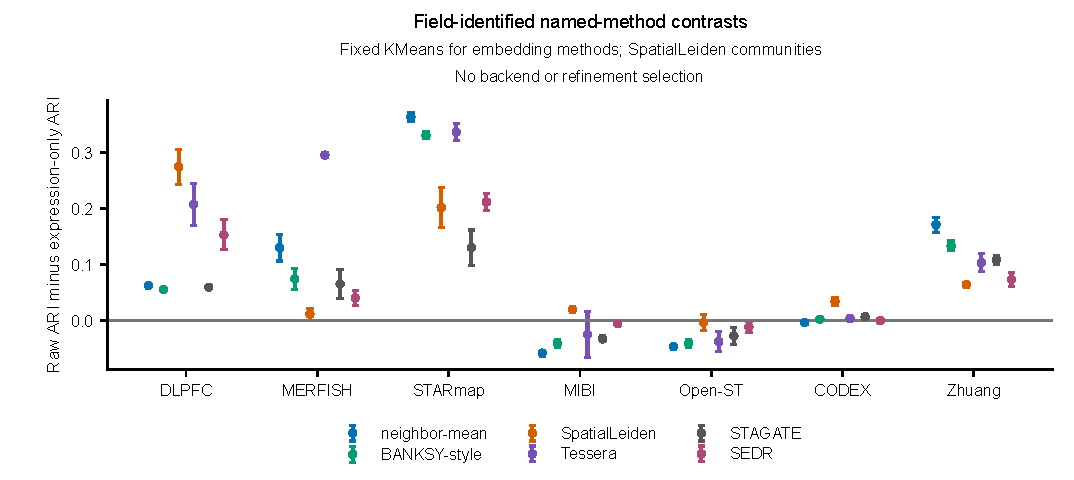
\includegraphics[width=\linewidth]{figs/fig_field_comparison.pdf}

\caption{Each named spatial method minus the genuinely expression-only comparator on the same cells and original seed identities. Dots are three-seed means; whiskers are the sample SD of the paired seed differences, not tissue-level confidence intervals. KMeans and raw assignments are fixed, so no true-label winner or refinement selection defines the contrast. Missing external methods are not imputed or included in an oracle maximum.}

\label{fig:field-comparison}\end{figure*}

Within-field contiguity is 0.486 for MIBI-TOF and 0.120 for CODEX in this labelled-neighbour definition. CODEX contains 15,454 labelled cells in the 16,000-cell model input; one labelled singleton contributes no contiguity term. These definitions explain why this value need not equal an earlier all-cell diagnostic. No coordinates are translated to manufacture field separation.

The matched neighbour-mean diagnostic isolates the graph consequence while holding features, PCA, KMeans and seed identities fixed. Pooling local frames gives mean ARI 0.032 on MIBI-TOF versus 0.153 within field, and -0.0001 versus 0.050 on CODEX. These are counterfactual audit arms, not inputs to the repaired comparator. They show that the coordinate error changes a model outcome as well as the contiguity axis.

Spatially refining the expression-only assignments changes its mean ARI by -0.036 to +0.148 across the retained objects. The sign is not fixed, and even a visually smoother control is no longer expression-only. The refinement counterfactual is stored separately and excluded from every named-method contrast (Fig.~\ref{fig:field-controls}).

\begin{figure*}[!htbp]\centering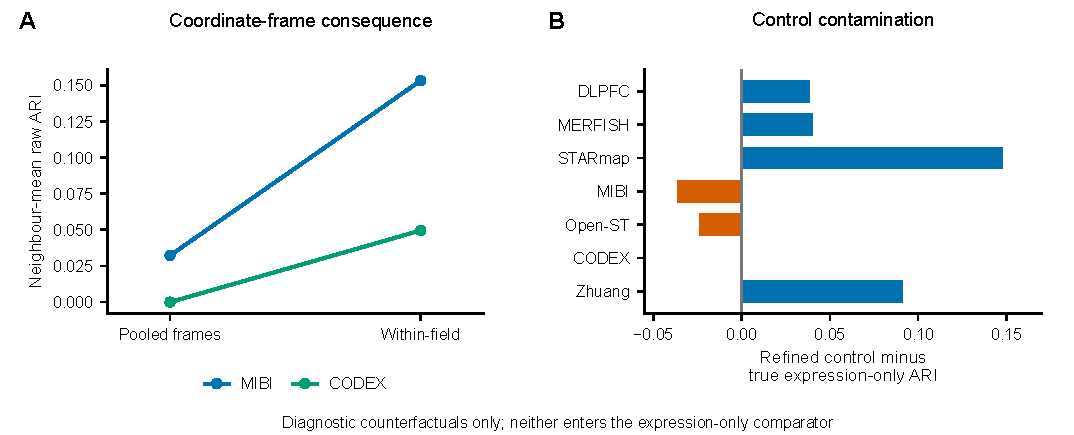
\includegraphics[width=\linewidth]{figs/fig_field_controls.pdf}

\caption{Direct consequences of two protocol errors, evaluated on the same inputs and seeds as the repaired analysis. (A) Three-seed mean neighbour-mean PCA--KMeans ARI with pooled local coordinates versus within-field coordinates for MIBI and CODEX. All other fitting settings are fixed. (B) Change in the nominal control's ARI if its expression-only labels are spatially refined. These diagnostic arms are not eligible controls, and no maximum across them is used.}

\label{fig:field-controls}\end{figure*}

Descriptive cross-object Spearman correlations between contiguity and the named contrasts range from 0.214 to 0.786; for Tessera it is 0.607 and for STAGATE 0.786. Field-chance adjustment leaves their ranks unchanged in this small set. These are method-specific summaries of seven selected objects, not confirmation of the old oracle correlation or of a deployment rule. Average-rank partial associations are row-order invariant but do not exclude confounding; no significance direction was an acceptance condition.
